\section{Event Reconstruction}
\label{sec:reconstruction}

Algorithms for converting Mu2e raw data into physics objects (i.e. reconstruction) have been in development for over 14 years. Operating on the output of the detailed simulations described in section \ref{sec:simulation}, these algorithms have been used to quantify the expected performance of the detector \cite{TDR} and the physics reach of the experiment \cite{Mu2e:2022ggl}. The output of reconstruction is used to perform the high-level calibration and alignment discussed in section \ref{sec:calibration}, and as the basis of the physics analysis processing described in section \ref{sec:analysis}. 

Reconstruction of the Mu2e primary event data stream proceeds in several stages. First, the low-level digital data (digis) coming from each Mu2e subsystem are converted into hit objects, which present the equivalent information in physical units, using calibration objects from the conditions service (see section~\ref{sec:databases}). A sequence of algorithms then aggregates and filters these hits into increasingly complete and accurate representations of physical particle candidates. The final versions of these particle candidates, with their ancillary information, are stored for downstream analysis. The reconstruction sequence relies on AI/ML at several stages, pointed out in the text.

Data from the extinction monitor and stopping target monitor are reconstructed in dedicated applications. Their final outputs will be recorded in the conditions database, associated with the corresponding event data by their intervals of validity. Reconstruction algorithms are currently under development.

All Mu2e reconstruction is implemented within the art framework~\cite{Green:2012gv}. Raw data from the DAQ system are stored as compressed digitizations with associated headers, called fragments, which are reformatted into Offline digi collections before reconstruction begins. Simulated data are produced directly as Offline digi collections. Individual reconstruction stages are implemented as art producer or filter modules. Wherever possible and applicable, standard utilities from stl, root GPL, and other public sources are used. Specialty codes, in particular the final Kalman filter track fit, are linked as external utilities.

\subsection{Tracker Hit Reconstruction}
The tracker digi data consists of separate TDC and Time Over Threshold (TOT) measurements from both ends of the straw and a digitized ADC waveform from the analog sum of the signals from the two straw ends. Raw data are zero-suppressed by requiring threshold crossings on both ends before readout. The TDC LSB and bin size calibration are defined in the digitization FPGA firmware. Each TDC values are separately converted to physical time using a linear function obtained from the conditions service, keyed on event ID and channel.
 
TOT is recorded online in units of readout clock ticks, counted from when the analog signal rises past threshold to when it falls below it. It is converted into an estimate of the drift time using a non-linear function obtained from the conditions service.
 
ADC waveforms are converted into an estimate of the deposited ionization energy from the particle crossing the straw. Several algorithms have been explored for this, including multi-peak fits to the waveform. By default, and in the trigger, the ionization energy is estimated by scaling the difference between the waveform maximum and the average of the waveform pre-samples (before the TDC threshold is crossed), which has been shown to be accurate in over 99\% of cases. Calibrations for electronic and physical gains are obtained from the conditions service, keyed by event ID and channel.

The reconstructed times, TOT, and ionization energy from each straw digitization are saved as straw hit objects. A downstream module averages hits in adjacent straws and close in time into a combined panel hit object. Panel hits provide a more accurate longitudinal position, and reduce the combinatorics of downstream algorithms. A subsequent module combines nearby panel hits in a tracker station into stereo hits, with more accurate position and some directional information. Straw, Panels, and Stereo hits all are represented by a single class so that downstream pattern recognition algorithms can pick the most appropriate to use without recoding.

The majority (>95\%) of reconstructed tracker hits come from beam pileup; isolated hits from photons, clusters of hits from spiraling $\delta$-rays and Compton electrons, and hits from Decay In Orbit (DIO) electrons and protons coming from stopped muons. 

A 2-D image of reconstructed hit positions from a typical Ce signal plus pileup event is shown in Fig.~\ref{fig:trackerhits}. The majority of these hits must be filtered out before tracks can be successfully found.
\begin{figure}[tbp]
 \centering
 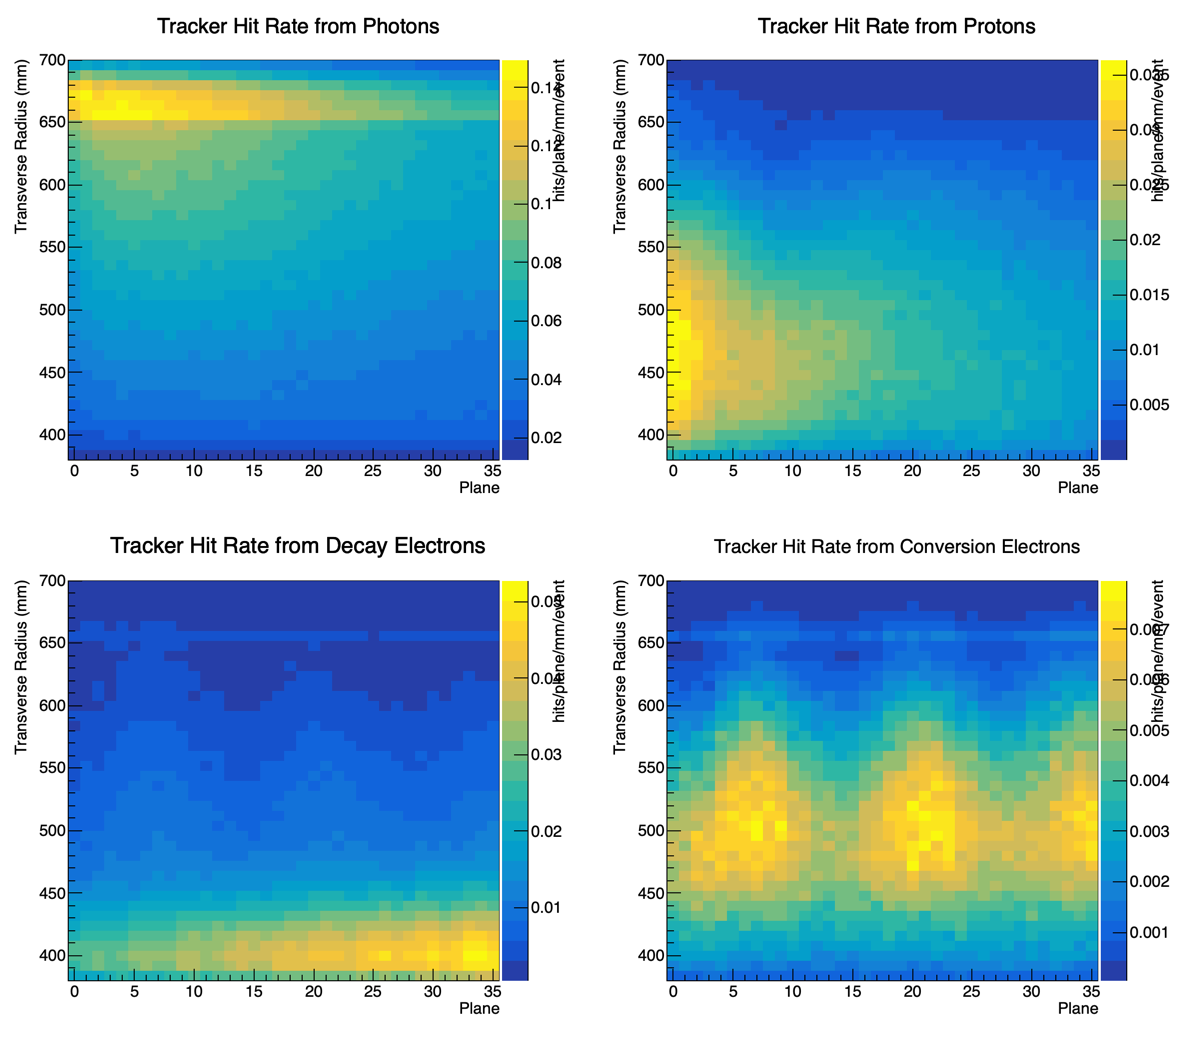
\includegraphics[width=\textwidth]{figures/trackerhits.png}%
 \caption{Track hit rate {\it vs} plane number and reconstructed transverse radius from different sources in simulated conversion electron events with beam pileup overlay.
 }%
 \label{fig:trackerhits}
\end{figure}

Hits from protons are removed using their large energy deposit. Hits from DIO are suppressed by requiring a minimum transverse radius, while hits originating from neutron capture in the DS are suppressed by requiring a maximum transverse radius. Hits from low-energy electrons are filtered using a dedicated algorithm that first clusters the hits in time and transverse position and then classifies the clusters using an ANN trained to separate low-energy from high-energy electrons by their geometric properties. The filtered hit collection passed to track pattern recognition has a signal purity of roughly 50\% in signal plus pileup simulation, inside the time window defined by the conversion electron hits.

\subsection{Signal Track Reconstruction}
The high-momentum track candidate search starts by looking for clusters of filtered hits with times within a sliding $\sim 50$ ns window. The hit time resolution is improved by roughly 30\% by subtracting the TOT-based drift time estimate. The hit straw Z position is used to correct the particle propagation time, dependent on the assumed or measured particle velocity.

Hits in a time cluster are passed to one of several helix finding algorithms, which extract rough helix parameters from the hit 3-D positions. Helix reconstruction is split into transverse (circle) and longitudinal phases, which are iterated between until convergence. One algorithm uses the position of high-energy (>50 \MeV) calorimeter clusters and the stopping target to seed the helix search, resulting in higher purity, but lower efficiency. The others use purely tracker information. Helices found by different algorithms that share the majority of their hits are merged. Helices from all algorithms use the same output data class. The performance of the different finding algorithms are similar, but not identical: in particular, the calorimeter-seeded algorithm is more robust against very high levels of pileup. As these algorithms are still being developed and tuned, and as they are easy to swap in and out and combine, Mu2e has not yet made a final decision on which ones will be used in the final trigger and reconstruction sequence.

Reconstructed helices are passed to a Kalman filter track fit to make final selections. The Mu2e fit uses the KinKal~\cite{Brown:2024tur} package, which is designed for precision kinematic reconstruction of low-momentum tracks in graded magnetic fields. The KinKal fit implements configurable simulated annealing, which allows for iterative pattern recognition and calibration refinement during the fit, and supports the integration of AI/ML pattern recognition tools as part of the fit. Within the KinKal framework, Mu2e has implemented a specialized track object, created fit constraint objects for both tracker hits and calorimeter clusters, and several ANN-based hit classification algorithms, which are applied as part of the annealing schedule. Associated calorimeter clusters are included as constraints on the fit time, allowing a more precise interpretation of the tracker hit drift time as a position constraint. The ANN classifiers remove residual background hits, refine the drift calibration, and help assign left-right ambiguities to tracker hits. 

Two configurations have been developed for the Mu2e KinKal fit, one optimized for use in the online trigger, and the other for offline analysis. The "trigger configuration" uses a minimal annealing schedule, a 1\% precision magnetic field correction, does not use track hit drift information, and does not add missing hits to the track. It provides a fit in roughly 5 msec/track processing time, with very high efficiency. The reconstructed momentum and the intrinsic momentum resolution using the trigger fit configuration for simulated conversion electron plus beam pileup events are shown in Fig.~\ref{fig:trigtrkmom}. Interpreting the full width half maximum (FWHM) of the momentum distribution as an effective core resolution using $\sigma = \rm FWHM/2.35$, the trigger fit achieves an absolute resolution of roughly $340 \keV$ down to the current trigger threshold of $80 \MeV$, which meets the Mu2e track trigger requirements~\cite{triggerreqs}.

\begin{figure}[tbp]
 \centering
 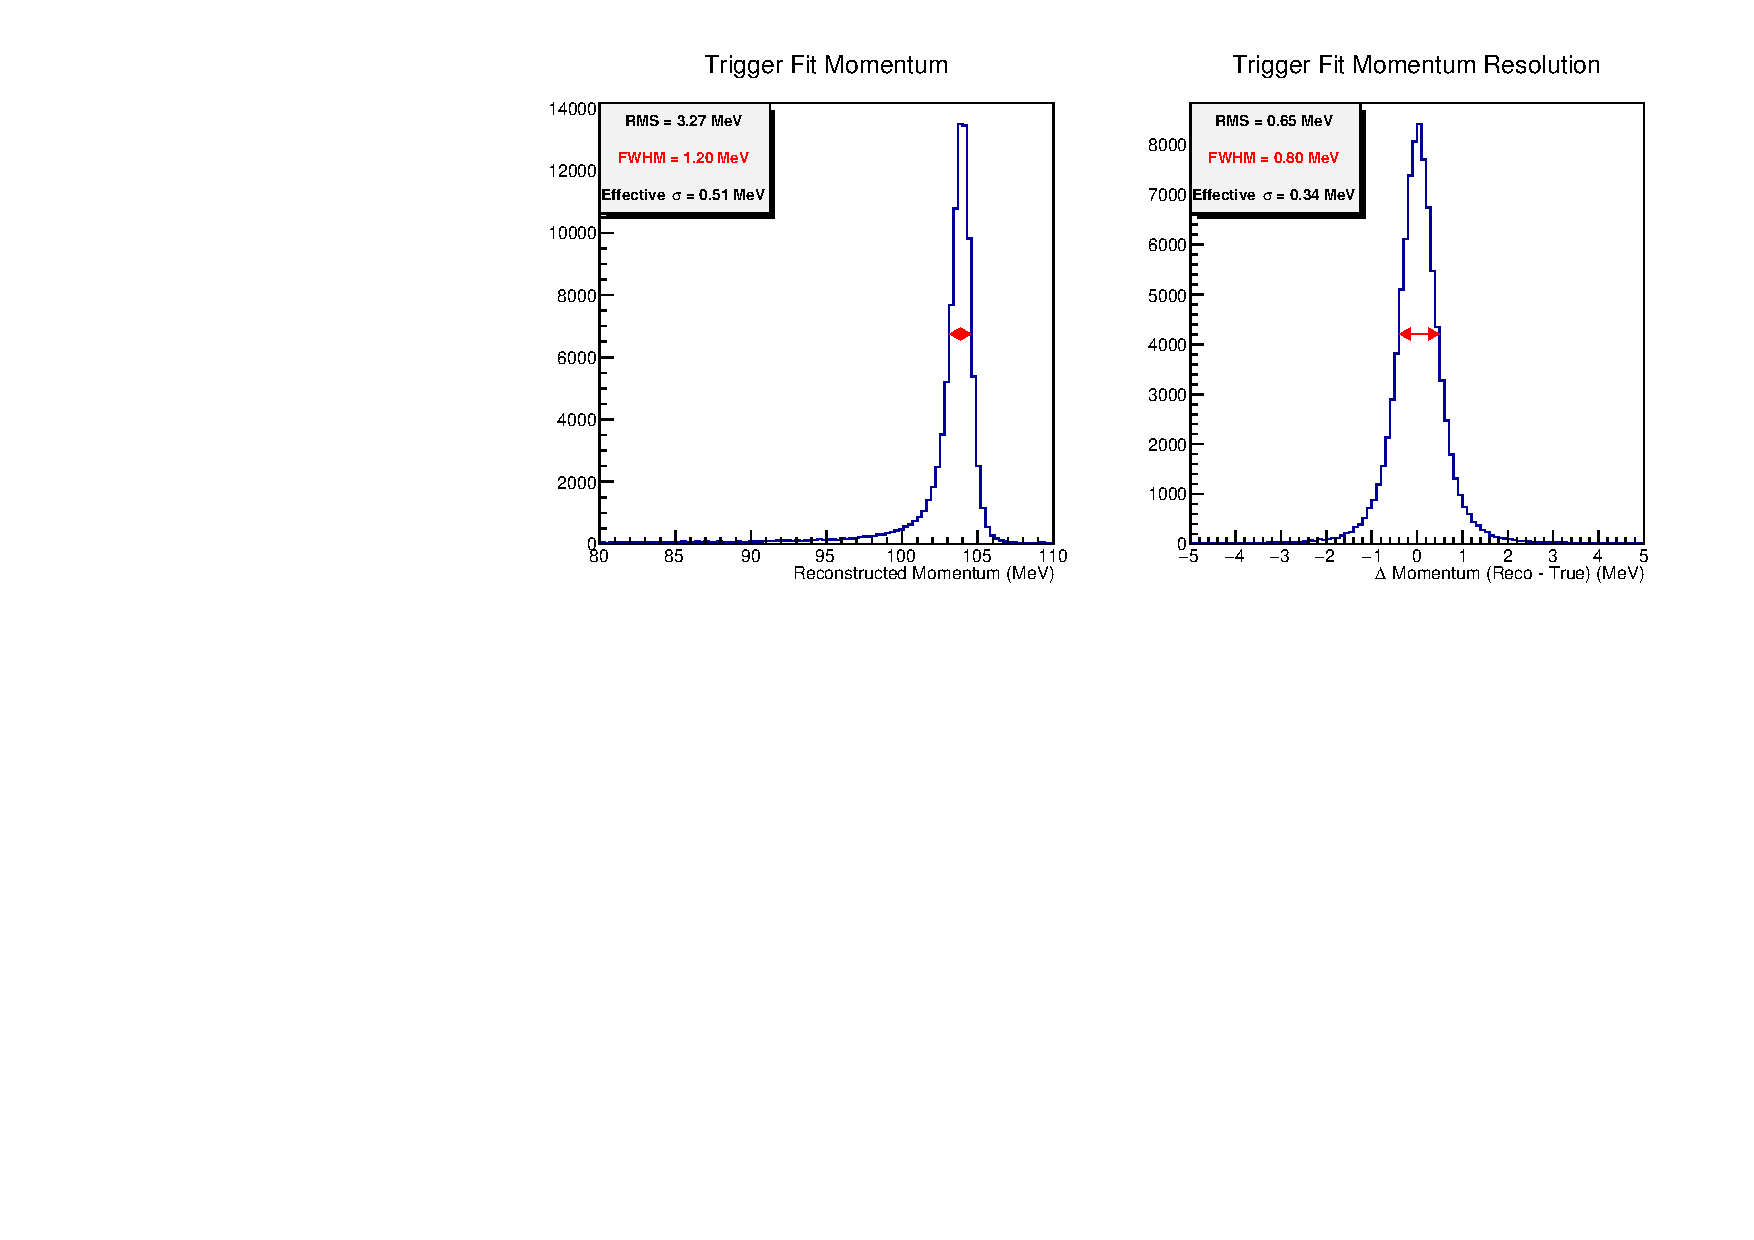
\includegraphics[width=\textwidth]{figures/KKTTmom.pdf}%
 \caption{Track momentum (left) and momentum resolution (right) in simulated conversion events with beam pileup overlay, reconstructed using the trigger KinKal configuration.}
 \label{fig:trigtrkmom}
\end{figure}

The "analysis configuration" uses a more gradual annealing schedule, a $10^{-4}$ precision magnetic field correction, full track hit drift information, and adds missing hits. This configuration requires roughly 50 msec/track, achieves essentially the same efficiency, and improved resolution. The reconstructed momentum and the intrinsic momentum resolution using the analysis fit configuration, sampled at the tracker entrance, for simulated conversion electron plus beam pileup events, are shown in Fig.~\ref{fig:anatrkmom}. 
%Interpreting the full width half maximum FWHM of the resolution distribution as an effective core resolution using $\sigma = FWHM/2.35$, we see 
The fit achieves an intrinsic resolution $\sigma = \rm FWHM/2.35 = 140 \keV$, exceeding the tracker requirement of $\sigma < 180 \keV$~\cite{trackerreqs}.

\begin{figure}[tbp]
 \centering
 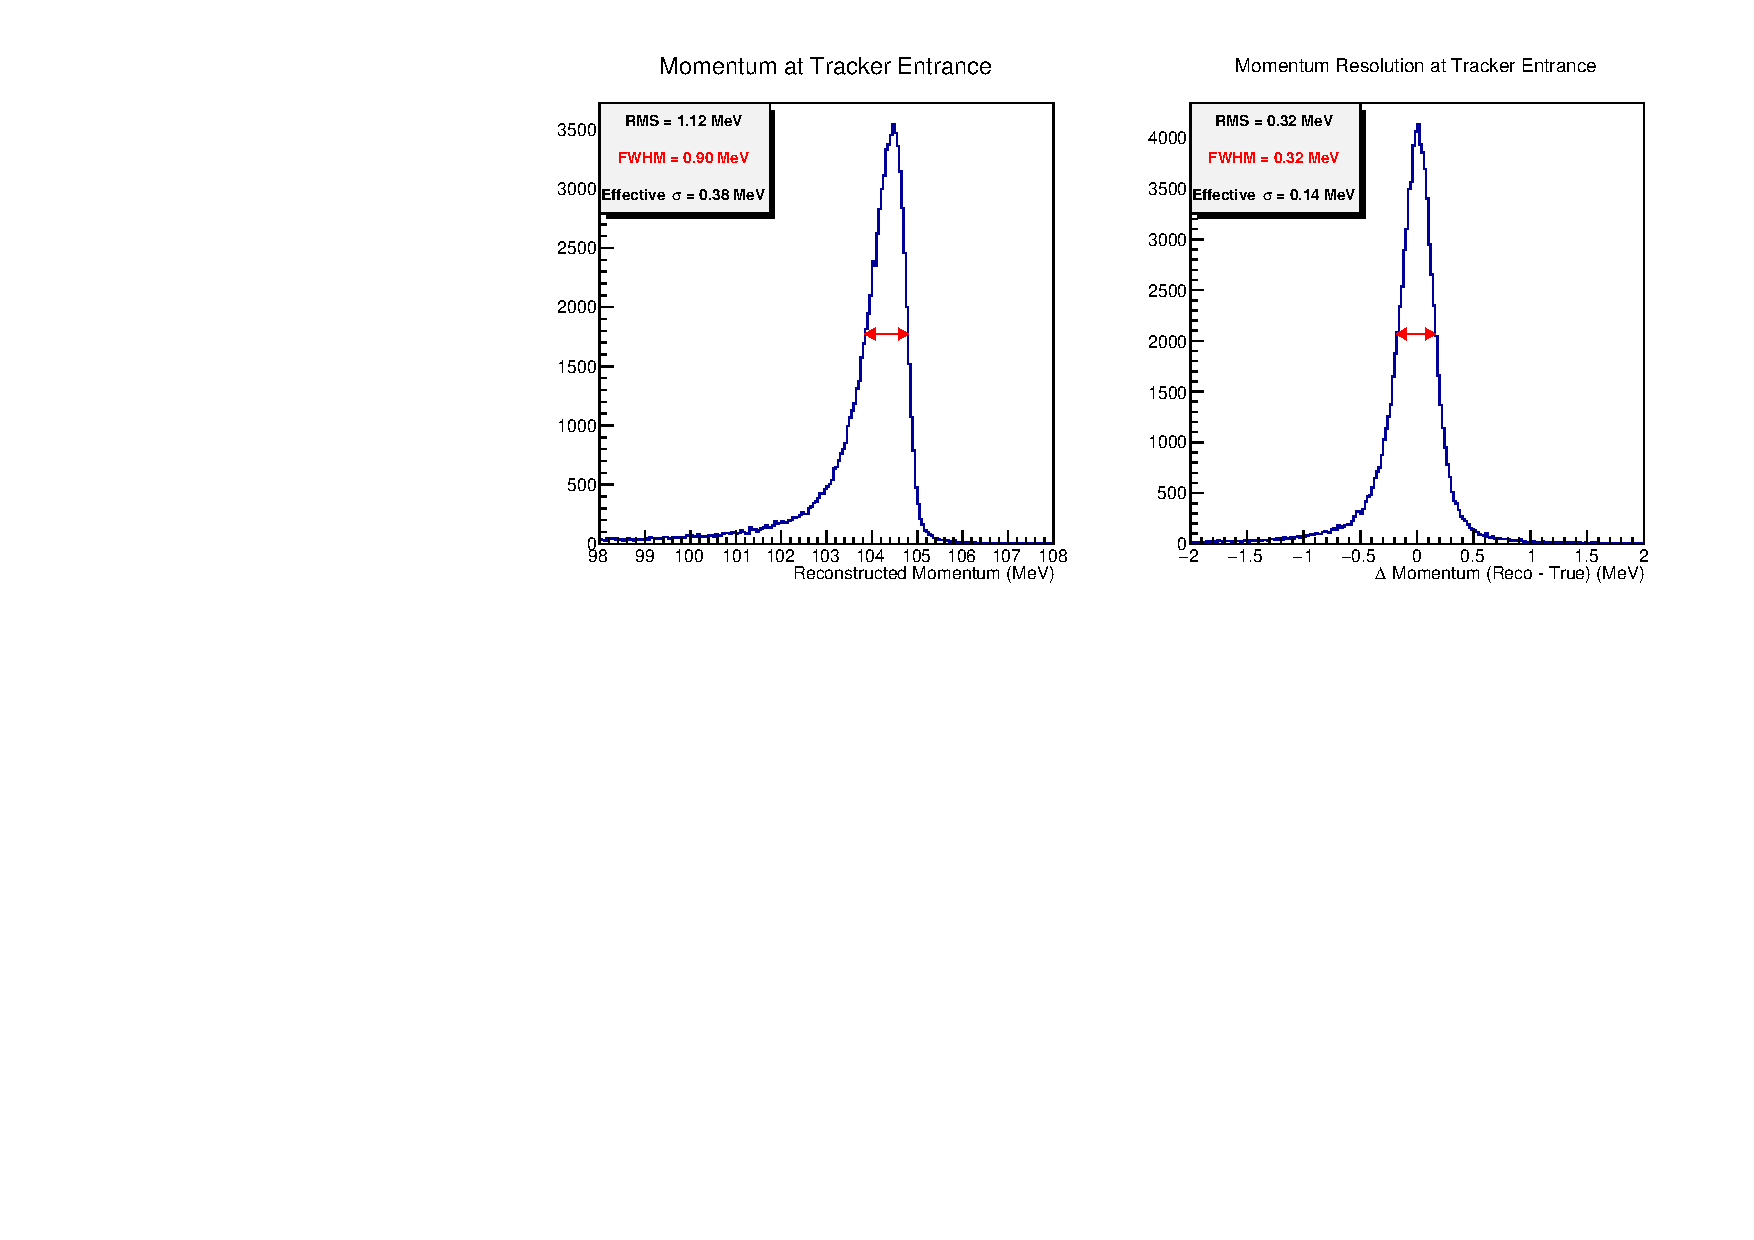
\includegraphics[width=\textwidth]{figures/KKMom.pdf}%
 \caption{Track momentum (left) and momentum resolution (right) sampled at the entrance to the tracker in simulated conversion events with beam pileup overlay, reconstructed using the analysis KinKal configuration (see text for definition).
 }%
 \label{fig:anatrkmom}
\end{figure}

As indicated by Fig.~\ref{fig:anatrkmom}, the absolute momentum resolution of Mu2e tracks is dominated by energy loss straggling in the stopping target and IPA. Evaluating the track momentum after extrapolation to the stopping target can potentially improve the absolute momentum resolution by accounting for estimated energy loss track-by-track instead of in aggregate. Algorithms to extrapolate reconstructed KinKal fit tracks beyond the fit region are under development. The core fit engine support for extrapolation is fully implemented and extrapolation in material-free regions has been demonstrated. The remaining task is the development of a KinKal model of the stopping target and IPA material and its integration with the fit.

\subsection{Straight Track Reconstruction}

The straight track reconstruction is used for cosmic ray tracks in the field-off configuration. As in the signal-track reconstruction, it begins by looking for clusters of filtered hits in time, but without attempting to correct for the particle propagation time. The straight line track seed also uses a simpler brute force algorithm. For each pair of straw hits, a straight line between the reconstructed hit positions is drawn and tested for intersections with the other hit straws, and the track with the highest number of successful intersections is chosen.

Two possible algorithms are used for the final reconstruction. First is a Kalman filter fit based on KinKal. Here the particle momentum is an input parameter that is held fixed during the fit. Similar to the signal fit, this fit can be configured to use a minimal annealing schedule and no drift information. In addition to making it faster, this configuration also makes it more robust against miscalibrations.

The second algorithm is a maximum likelihood fit that uses the ROOT Minuit2 minimizer. The likelihood for each straw hit includes both drift and longitudinal information, with the drift time likelihood for a given drift radius given by an exponentially modified Gaussian distribution that models the effect of both the random variations of the drift times for a single cluster and the exponential distribution of the effective drift distance given the discrete cluster statistics. The track is parameterized as a perfect straight line so no scattering is included. As a global fit, the results from this algorithm can easily be used with the Millepede-II alignment algorithm. 

\subsection{Calorimeter Reconstruction}

The data written by the calorimeter front-end electronics contains zero-suppressed waveforms recorded by the photo-sensors at the back of each crystal. These waveforms could be produced by a single or several particles depositing energy in a crystal during a short amount of time. In the latter case, the recorded waveform contains overlapping peaks, exhibiting multiple local maxima. The signal extraction procedure starts by fitting the waveform with an iterative procedure to extract the time and amplitude of each peak. The fit model is revised by adding or removing peaks until the chi-squared of the fit falls below a specified threshold (up to nine peaks can be extracted in a single waveform). The leading edge of the first peak is also refit to improve the timing resolution. The signal amplitudes are converted into energy deposits by using photosensor-specific calibration constants. The outputs of two photo-sensors within a time window of 4 ns are then merged to form crystal hits. 

Calorimeter clusters are finally formed by combining crystal hits. The most energetic hit is taken as a cluster seed, and all simply connected hits compatible with the seed time are added to the cluster content. These hits are then removed from the pool of available hits, and the procedure is repeated until all hits have been assigned to a cluster. A fraction of the particles interacting with the calorimeter produces one or more low-energy clusters near a more energetic one. A procedure is applied to combine these split-off clusters with the main cluster and improve the energy resolution. The energy, time, and other properties of the clusters are finally determined.

\subsection{CRV Reconstruction}
The CRV front-end boards record waveforms of each channel of the CRV detector. This is done in a non-zero-suppressed mode and a zero-suppressed mode, where the zero suppression threshold will be at around 5.5 photo-electrons. Non-zero-suppressed data is used for calibration purposes, and to validate the zero-suppression algorithm.

The zero-suppressed waveform data is used to reconstruct candidates of cosmic rays going through the CRV. First, individual waveforms are searched for pulses (local maxima), extracting the pulse time and pulse area. The pulse area is normalized by a channel-specific calibration constant (extracted from the conditions database) to obtain an estimate of the number of photo-electrons in this pulse.
%To distinguish CRV pulses that are caused by cosmic rays entering the detector (and may cause conversion-like electrons) from CRV pulses of other sources (e.g. beam-induced tracks), pulses in locally adjacent 
Based on the time, number of photo-electrons, and location of recorded CRV pulses, groups of pulses are associated with coincidence clusters. The current coincidence criterion requires pulses in 3 out of 4 CRV layers, with at least 10 photo-electrons, within 20 ns. Conversion electron candidates consistent in time and space with originating from a CRV coincidence cluster will be rejected (vetoed) in analysis. %Current algorithms achieve XXX rejection rate with a cost of YYY in signal candidate acceptance.
The CRV coincidence criteria and track consistency algorithms remain to be optimized for maximal acceptance while keeping the expected number of cosmic background tracks well below one.

\subsection{STM Reconstruction}
The STM data written by the DAQ consists of prescaled unsuppressed and zero-suppressed digitized waveforms as well the outputs of the online pulse processing algorithm, which consist of the uncalibrated energy and time of each hit. The unsuppressed and zero-suppressed waveforms are used to validate the online algorithms, and the outputs of the pulse-processing algorithms are used for the analysis. The pulse-processing algorithms have been tested at high rates using data collected in a test beam setup.

The outputs of the pulse-processing algorithms are calibrated in the Offline framework with calibration constants stored in the conditions service. We plot the energy spectrum of the calibrated hits and fit Gaussian functions to the peaks of interest in order to estimate the number of stopped muons. This method achieves a 10\% statistical uncertainty on the number of stopped muons with $\sim 10$ minutes of data in simulation. These $\sim$10-minute counts and associated uncertainties will be stored in a database. Event-by-event information such as the number of tracker hits or the total energy deposit in the calorimeter, can be used to interpolate between STM measurements to estimate the number of stopped muons per event.

\subsection{Extinction Monitor Reconstruction}

The reconstruction starts by grouping adjacent pixel hits from the same clock tick into clusters. The coordinates of a cluster are computed as the center of gravity of its component hits. The next step is pattern recognition. Straight line tracklets are formed from clusters in the upstream and, independently, downstream sensor stacks. A tracklet is constructed from 3 clusters; all in the same clock tick but in different planes. The position cuts are loose, allowing for a pixel-size misalignment error and a multiple scattering angle of up to 5 mrad in a plane. Upstream and downstream tracklets are matched into candidate tracks if they are in the same clock tick and if the angle difference in the non-bend projection for the tracklets is within $0.005$. A $\chi^2$ fit is performed on candidate tracks to determine 5 parameters: the starting position $(x,y)$ and direction at the detector entrance, and the bend radius in the magnet. 
%Figure~\ref{fig:extmonEff} Shows the extinction monitor track reconstruction efficiency as a function of particle multiplicity in simulation.
%\begin{figure}[tbp]
% \centering
% 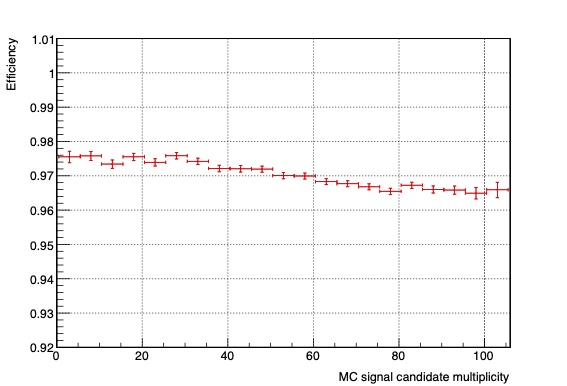
\includegraphics[width=\textwidth]{figures/extmonEff.png}%
% \caption{Track reconstruction efficiency vs particle multiplicity.
% }%
% \label{fig:extmonEff}
%\end{figure}

